% KU Leuven latex presentation template
%
% © 2012 Michael Hofmann
%
% This work is licensed under the Creative Commons Attribution 3.0 Unported License.
% To view a copy of this license, visit
% http://creativecommons.org/licenses/by/3.0/ or send a letter to Creative
% Commons, 444 Castro Street, Suite 900, Mountain View, California, 94041, USA.

\documentclass[t,12pt,english
\ifx\beamermode\undefined\else,\beamermode\fi
]{beamer}
%\setbeameroption{show notes}
%\setbeameroption{show only notes}

\usepackage[utf8]{inputenc}
\usepackage[T1]{fontenc}
\usepackage{amsmath}
\usepackage[nohyperlinks]{acronym}
\usepackage{babel,lmodern,graphicx,mathptmx,xspace,wasysym,microtype,booktabs,tabularx,relsize,textcomp,longtable,lipsum,colortbl,eurosym,url,multicol,etoolbox,multimedia,pdfpages,fixltx2e,ifluatex,epstopdf}
\usepackage[olditem,oldenum]{paralist}
\usepackage[babel=true]{csquotes}
\usepackage[thinqspace,amssymb,textstyle]{SIunits}
\usepackage[textsize=tiny]{todonotes}
\usepackage[symbol]{footmisc}
\usepackage[notquote]{hanging}
\usepackage[normalem]{ulem}
%\usepackage{lua-visual-debug}

\pdfstringdefDisableCommands{\renewcommand{\sout}{}}
\graphicspath{{Images4/}}
% Fix sort order in case the same file exists with multiple extensions
\DeclareGraphicsExtensions{.pdf,.png,.jpeg,.jpg,.eps}
\frenchspacing

\input{templates/definitions.tex}



%% From pandoc default template
%% End pandoc

\mode<presentation>

%\hypersetup{pdfpagemode=FullScreen}

\definecolor{kuldefault}{HTML}{00407a}
\definecolor{kulbright}{HTML}{52bdec}
\definecolor{kulleft}{HTML}{1d8db0}
\definecolor{kulright}{HTML}{116e8a}

\definecolor{kulyellow}{HTML}{BC8F00}
\definecolor{kulorange}{HTML}{BC6E00}
\definecolor{kulgreen}{HTML}{007F4F}
\definecolor{kulred}{HTML}{FF4422}

\setbeamercolor{structure}{fg=kulbright}
\setbeamercolor{title}{fg=white}
\setbeamercolor{footline}{parent=title}
\setbeamercolor{normal text}{fg=kuldefault}
\setbeamercolor{item}{parent=normal text}
\setbeamercolor{section in toc}{parent=normal text}
\setbeamerfont{title}{size=\Large}
\setbeamerfont{tiny structure}{series=\bfseries}
\setbeamerfont{caption}{}

\setbeamersize{text margin left=0.8cm}
\setbeamersize{text margin right=0.8cm}
\setbeamersize{sidebar width left=0cm}

\setbeamertemplate{navigation symbols}{}
\setbeamertemplate{itemize item}{\footnotesize\raise1pt\hbox{\textbullet}}
\setbeamertemplate{itemize subitem}{--}
\setbeamertemplate{itemize subsubitem}{\tiny\raise1.5pt\hbox{\textbullet}}

\setlength\leftmargini{1em}
\setlength\leftmarginii{1em}
\setlength\leftmarginiii{1em}

\defbeamertemplate{background canvas}{title}
{%
    \pgfdeclarehorizontalshading{bgshading}{8.70cm}{color(0cm)=(kulleft); color(\the\paperwidth)=(kulright)}%
    \vbox to 8.70cm{%
        \pgfuseshading{bgshading}\hspace*{-1.6cm}%
    }%
    \hskip-\paperwidth%
    \hskip1.6cm%
    \vbox to \paperheight{%
        \vskip0.5cm\hskip0.5cm\includegraphics[width=2.83cm]{templates/kuleuven}%
        \vskip0.99cm\hskip0.76cm\includegraphics[width=2.84cm]{templates/key}%
        \vskip-0.57cm\hskip11.61cm\includegraphics[width=0.58cm]{templates/sedes}\hspace*{-1cm}%
        \vfill
    }%
}

\defbeamertemplate{background canvas}{grid}
{%
    \begin{tikzpicture}[remember picture,overlay,every node/.style={anchor=center}]
        \foreach \d in {0,...,20} {
            \draw[gray] (\d,0) -- (\d,-20);
            \draw[gray] (0,-\d) -- (20,-\d);
            \draw[lightgray] (\d+0.5,0) -- (\d+0.5,-20);
            \draw[lightgray] (0,-\d-0.5) -- (20,-\d-0.5);
            \node[anchor=north,red,font=\tiny] at (\d,0) {\d};
            \node[anchor=west,red,font=\tiny] at (0,-\d) {\d};
        }
    \end{tikzpicture}
}

\defbeamertemplate{background canvas}{plain}{}

\defbeamertemplate{footline}{large}
{%
    \pgfdeclarehorizontalshading{bgshading}{0.62cm}{color(0cm)=(kulleft); color(\the\paperwidth)=(kulright)}%
    \vskip.3cm% make room for the logo
    \parbox[t][0.62cm]{\paperwidth}{\pgfuseshading{bgshading}}\par%
    \vskip-0.62cm%
    \begin{beamercolorbox}[ht=0.37cm,dp=0.25cm,center]{page number in head/foot}%
    \insertframenumber%
    \end{beamercolorbox}%
    \vskip-0.92cm%
    \parbox[t][0.92cm]{\paperwidth}{\hskip10.33cm\includegraphics[width=2.10cm]{templates/kuleuven}}\par%
}

\defbeamertemplate{footline}{nopagenumber}
{%
    \pgfdeclarehorizontalshading{bgshading}{0.62cm}{color(0cm)=(kulleft); color(\the\paperwidth)=(kulright)}%
    \vskip.3cm% make room for the logo
    \parbox[t][0.62cm]{\paperwidth}{\pgfuseshading{bgshading}}\par%
    \vskip-0.62cm%
    \begin{beamercolorbox}[ht=0.37cm,dp=0.25cm,center,ignorebg]{page number in head/foot}%
    %
    \end{beamercolorbox}%
    \vskip-0.92cm%
    \parbox[t][0.92cm]{\paperwidth}{\hskip10.33cm\includegraphics[width=2.10cm]{templates/kuleuven}}\par%
}

\defbeamertemplate{footline}{small}
{%
    \vskip.3cm% make room for the logo
    \begin{beamercolorbox}[ht=0.37cm,dp=0.25cm,center,ignorebg]{normal text}%
    \mdseries\insertframenumber%
    \end{beamercolorbox}%
}

\setbeamertemplate{footline}[large]

\setbeamertemplate{frametitle}
{%
    \nointerlineskip%
    \vskip.28cm%
    {\usebeamercolor[fg]{framesubtitle}\usebeamerfont{framesubtitle}\insertsupertitle\strut\par}%
    \vskip-.2cm%
    {\usebeamercolor[fg]{frametitle}\usebeamerfont{frametitle}\insertframetitle\strut\par}%
    \vskip-.3cm%
}

\setbeamertemplate{title page}
{
    \vbox{}%
    \vskip2.8cm%
    \vbox to 6.5cm{%
        \hskip2.8cm%
        \begin{minipage}{7.9cm}
            \begin{beamercolorbox}{title}
                \usebeamerfont{title}%
                \inserttitle\par%
                \ifx\insertsubtitle\undefined%
                \else%
                    \vskip0.25em%
                    {\usebeamerfont{subtitle}\usebeamercolor[fg]{subtitle}\insertsubtitle\par}%
                \fi%
            \end{beamercolorbox}%
            \vskip1em\par
            \begin{beamercolorbox}{author}
                \usebeamerfont{author}\usebeamercolor[fg]{subtitle}%
                \insertauthor
            \end{beamercolorbox}
            \begin{beamercolorbox}{institute}
                \usebeamerfont{institute}\usebeamercolor[fg]{subtitle}%
                \insertinstitute
                \end{beamercolorbox}
            \begin{beamercolorbox}{date}
                \usebeamerfont{date}\usebeamercolor[fg]{subtitle}%
                \insertdate
            \end{beamercolorbox}%
        \end{minipage}%
        \vfill
    }
}

\mode<all>

\newcommand{\inlinesound}[2]{\movie[inlinesound,encoding=Signed,samplingrate=44100]{#1}{#2}}

% disable for now as otherwise all commands that go between frames generated by
% the filter will result in duplicate toc lines
\renewcommand{\addcontentsline}[3]{}

\newcommand{\largefooter}{\setbeamertemplate{footline}[large]}
\newcommand{\emptyfooter}{\setbeamertemplate{footline}[nopagenumber]}
\newcommand{\smallfooter}{\setbeamertemplate{footline}[small]}

\newcommand{\sectiontoc}{\AtBeginSection[]{{
    \nosupertitle
    \emptyfooter
    \begin{frame}[noframenumbering]{Outline}
                \tableofcontents[currentsection]
            \end{frame}
    \largefooter
}}}

\newcommand{\subsectiontoc}{\AtBeginSubsection[]{{
    \nosupertitle
    \emptyfooter
    \begin{frame}[noframenumbering]{Outline}
                \tableofcontents[currentsection,currentsubsection]
           \end{frame}
    \largefooter
}}}

\newcommand{\notoc}{\AtBeginSection[]{}\AtBeginSubsection[]{}}

\newcommand{\nosupertitle}{\renewcommand{\insertsupertitle}{}}
\newcommand{\sectiontitle}{\renewcommand{\insertsupertitle}{\insertsectionhead}}
\newcommand{\subsectiontitle}{\renewcommand{\insertsupertitle}{\insertsectionhead\ifx\insertsubsectionhead\empty\else{} -- \insertsubsectionhead\fi}}

% animations do not work atm as figures are set on independent frames
\newcommand{\slidefig}[2]{\usebackgroundtemplate{\parbox[c][\paperheight][c]{\paperwidth}{\centering\includegraphics#1[height=\paperheight,width=\paperwidth,keepaspectratio]{#2}}}\begin{frame}[plain]\end{frame}\usedefaultcanvas}

\newcommand{\usedefaultcanvas}{\setbeamertemplate{background canvas}[\defaultcanvas]}
\newcommand{\gridcanvas}{\renewcommand{\defaultcanvas}{grid}\usedefaultcanvas}
\newcommand{\plaincanvas}{\renewcommand{\defaultcanvas}{plain}\usedefaultcanvas}

\newcommand{\insertsupertitle}{}






\newcommand{\defaultcanvas}{plain}


% Defining a new coordinate system for the page:
%
% ----------------
% |(0,1)    (1,1)|
% |              |
% |(0,0)    (1,0)|
% ----------------
\makeatletter
\def\parsecomma#1,#2\endparsecomma{\def\page@x{#1}\def\page@y{#2}}
\tikzdeclarecoordinatesystem{page}{
    \parsecomma#1\endparsecomma
    \pgfpointanchor{current page}{north east}
    % Save the upper right corner
    \pgf@xc=\pgf@x%
    \pgf@yc=\pgf@y%
    % save the lower left corner
    \pgfpointanchor{current page}{south west}
    \pgf@xb=\pgf@x%
    \pgf@yb=\pgf@y%
    % Transform to the correct placement
    \pgfmathparse{(\pgf@xc-\pgf@xb)*\page@x+(\pgf@xb)}
    \expandafter\pgf@x\expandafter=\pgfmathresult pt
    \pgfmathparse{(\pgf@yc-\pgf@yb)*\page@y+(\pgf@yb)}
    \expandafter\pgf@y\expandafter=\pgfmathresult pt
}
\makeatother

% Example:
%\begin{tikzpicture}[remember picture,overlay,every node/.style={anchor=center}]
%  \node at (page cs:0.5,0.3) {0.5,0.3};
%  \node at (page cs:0,0) {0,0};
%  \draw(page cs:0,0) -- (page cs:1,1);
%  \draw[thick,red] (page cs:0,0) rectangle (page cs:1,1);
%  \draw[thick,green] (page cs:0.2,0.2) rectangle (page cs:0.8,0.8);
%\end{tikzpicture}

\setcounter{secnumdepth}{0}

\title{Source localization}
\subtitle{\tiny Biomedical Data Procession part II}
\author{\\ \href{vangjush.komini@uzleuven.be}{\textbf{\textit{Vangjush Komini}}}
}


\institute{{\tiny }\vspace{.10cm} }
\date{\href{www.kul.be}{KU Leuven}\\ \vspace{.10cm}\today}

\begin{document}

\setbeamertemplate{background canvas}[title]

\begin{frame}[plain,noframenumbering]
    \titlepage
\end{frame}

\usedefaultcanvas


\emptyfooter
\begin{frame}[noframenumbering]{Outline}
        \tableofcontents
    \end{frame}
\largefooter

\section{Forward problem}\label{first-section}

\begin{frame}{Electrode placement in the head}


\begin{figure}[!htbp]
\centering
\includegraphics[width=.5\textwidth]{1.jpg}
\end{figure}

\end{frame}


\begin{frame}{Dipole placed between the center of the head and the right ear}

\begin{figure}[!htbp]
\minipage{.5\textwidth}%
\centering
\includegraphics[width=1\textwidth]{2.jpg}
\endminipage\hfill
\minipage{.5\textwidth}%
\centering
\includegraphics[width=1\textwidth]{3.jpg}
\endminipage\hfill
\end{figure}

\end{frame}


\begin{frame}{Voltage distribution created from the central dipole}

\begin{figure}[!htbp]
\minipage{.5\textwidth}%
\centering
\includegraphics[width=1\textwidth]{4.jpg}\\
\tiny{Voltage distribution along the electrodes}\label{a2}
\endminipage\hfill
\minipage{.5\textwidth}%
\centering
\includegraphics[width=1\textwidth]{5.jpg}\\
\tiny{Dipole placed at the center oriented along the right ear}\label{a1}
\endminipage\hfill
\end{figure}

\end{frame}


\begin{frame}{Lead field matrix plots respectively to the columns}



\begin{figure}[!htbp]
\minipage{.33\textwidth}%
\centering
\includegraphics[width=1\textwidth]{6.jpg}\\
\tiny{Lead field matrix along the x axis which is exactly as the the real voltage distribution of the main dipole}
\endminipage\hfill
\minipage{.33\textwidth}%
\centering
\includegraphics[width=1\textwidth]{7.jpg}\\
\tiny{Lead filed matrix plot for the middle column along the y axis}
\endminipage\hfill
\minipage{.33\textwidth}%
\centering
\includegraphics[width=1\textwidth]{8.jpg}\\
\tiny{Lead filed matrix plot for the middle column along the y axis}
\endminipage\hfill
\end{figure}
    
\end{frame}


\begin{frame}{Superposition of dipoles}


\begin{figure}[!htbp]
\minipage{.5\textwidth}%
\centering
\includegraphics[width=1\textwidth]{9.jpg}
\endminipage\hfill
\minipage{.5\textwidth}%
\centering
\includegraphics[width=1\textwidth]{10.jpg}
\endminipage\hfill
\end{figure}

\tiny{The voltage from both dipoles at the center where the first one directed along x the other one is oriented along z axis}

\end{frame}

\begin{frame}{EEG signal simulated }
 

\begin{figure}[!htbp]
\minipage{.5\textwidth}%
\centering
\includegraphics[width=1\textwidth]{11.jpg}\\
\tiny{EEG simulated from the dipole placed at an arbitrary place in the brain rotating along xy plane }
\endminipage\hfill
\minipage{.5\textwidth}%
\centering
\includegraphics[width=1\textwidth]{12.jpg}\\
\tiny{Dipole location and orientation in the brain rotated along xy plane}
\endminipage\hfill
\end{figure}

\end{frame}



\section{Inverse problem}

\begin{frame}{Estimation of dipole using a single time instance}

\begin{figure}[!htbp]
\minipage{.33\textwidth}%
\centering
\includegraphics[width=1\textwidth]{13.jpg}\\
\tiny{RRE for different simulation}
\endminipage\hfill
\minipage{.33\textwidth}%
\centering
\includegraphics[width=1\textwidth]{14.jpg}

\endminipage\hfill
\minipage{.33\textwidth}%
\centering
\includegraphics[width=1\textwidth]{15.jpg}

\endminipage\hfill
\minipage{.33\textwidth}%
\centering
\includegraphics[width=1\textwidth]{16.jpg}
\endminipage\hfill
\minipage{.33\textwidth}%
\centering
\includegraphics[width=1\textwidth]{17.jpg}

\endminipage\hfill
\minipage{.33\textwidth}%
\centering
\includegraphics[width=1\textwidth]{18.jpg}

\endminipage\hfill
\tiny{Voltage estimation of the inverse problem}
\end{figure}
    
\end{frame}


\begin{frame}{Estimation overview}

\begin{table}[!htbp]
\tiny
\centering
\caption{\small Orientation}
\begin{tabular}{c c c c c c c c c c c c c c c c c c c c c c c c c c c c c c c } 
   \hline 
$ $&$x$&$y$&$z$\\
   \hline 
$ Orig$&$1$&$0$&$0$\\
$1$&$0.0021339 $&$-0.31206$&$ 0.19721$\\
$2$&$ 0.0042572$&$ -0.88824$&$   0.52397$\\
$3$&$-8.1962e-06$&$-3.278e-06$&$  1.5082e-05$\\
$4$&$-8.1572e-08$&$2.0502e-05$&$1.7784e-05$\\
$5$&$1.0203e-05$&$3.0967e-05$&$2.7826e-05$\\
\hline 

\end{tabular}
\end{table}


 \begin{table}[!htbp]
 \tiny
\centering
\caption{\small Location}
\begin{tabular}{c c c c c c c c c c c c c c c c c c c c c c c c c c c c c c c } 
   \hline 
$ $&$x$&$y$&$z$\\
   \hline 
$ Orig$&$0.06$&$0$&$0.01$\\
$1$&$0.063348$&$-0.0027615$&$-0.048778$\\
$2$&$0.025834$&$0.00053067$&$-0.075711$\\ 
$3$&$0.060001$&$1.4583e-06 $&$0.010002$\\
$4$&$0.059999$&$1.451e-08$&$0.0099958 $\\
$5$&$0.059999$&$-1.815e-06$&$0.0099949 $\\
\hline 

\end{tabular}
\end{table}


\end{frame}

\subsection{Error estimation for two different electrode malfunctioning}

\begin{frame}{Error due to the electrode}

\begin{figure}[!htbp]
\minipage{.33\textwidth}%
\centering
\includegraphics[width=1\textwidth]{19.jpg}\\
\tiny{Measurement with all the electrodes}
\endminipage\hfill
\minipage{.33\textwidth}%
\centering
\includegraphics[width=1\textwidth]{20.jpg}\\
\tiny{Measurement with the electrodes P8 down}
\endminipage\hfill
\minipage{.33\textwidth}%
\centering
\includegraphics[width=1\textwidth]{21.jpg}\\
\tiny{Measurement with the electrodes F7 down}
\endminipage\hfill
\end{figure}

\begin{figure}[!htbp]
\minipage{.33\textwidth}%
\centering
\includegraphics[width=1\textwidth]{54.jpg}\\
\tiny{All electrodes working}
\endminipage\hfill
\minipage{.33\textwidth}%
\centering
\includegraphics[width=1\textwidth]{23.jpg}\\
\tiny{P8}\label{A23}
\endminipage\hfill
\minipage{.33\textwidth}%
\centering
\includegraphics[width=1\textwidth]{34.jpg}\\
\tiny{P8-F7}\label{34}
\endminipage\hfill
\caption{\small \tiny Error estimation for two different electrode malfunctioning}
\end{figure}


\end{frame}

\begin{frame}{Overview of the results for electrode malfunctioning}

 \begin{table}[!htbp]
 \tiny 
\centering
\caption{\small Estimation of the dipoles}
\label{table:5}
\begin{tabular}{c c c c c c c c c c c c c c c c c c c c c c c c c c c c c c c } 
\hline 
$ $&$x$&$y$&$z$&$dx$&$dy$&$dz$\\
\hline 
$Orig$&$0.06$&$0$&$0.01$&$1$&$0$&$0$\\
\hline 
$1$&$0.02238$&$1.9923e-05$&$0.025523$&$0.99137$&$-4.0055e-05$&$-0.13107$\\
$2$&$0.022421$&$-3.3486e-07$&$0.025489$&$0.99142$&$6.72e-07$&$-0.13072$\\
$3$&$0.022396$&$ -4.8086e-05$&$0.025531$&$0.99138$&$9.659e-05$&$-0.131$\\
$4$&$0.022404$&$2.9814e-05$&$0.025493$&$0.99141$&$-5.9878e-05$&$-0.13083$\\
$5$&$0.022386$&$-1.9192e-05$&$0.025448$&$0.99141$&$3.859e-05$&$ -0.13078$\\
$1$&$0.062968$&$-0.0037903$&$ -0.0492$&$0.91144$&$0.0041816$&$-0.41141$\\
$2$&$0.062871$&$-0.0014755$&$ 0.016217$&$0.99902$&$0.015062$&$-0.041705$\\
$3$&$0.062876$&$-0.0014806$&$ 0.016246$&$0.99901$&$0.015078$&$-0.041917$\\
$4$&$0.06286$&$-0.0015184$&$0.016184$&$0.99902$&$0.015267$&$-0.04156$\\
$5$&$0.062892$&$-0.0014951$&$ 0.016281$&$0.999$&$0.015125$&$-0.041993$\\
\hline 

\end{tabular}
\end{table}

    
\end{frame}


\subsection{Error from the  conductivity tissue}

\begin{frame}{Random dipole distribution}
 
\begin{table}[!htbp]
\tiny
\centering
\begin{tabular}{c c c c c c c c c c c c c c c c c c c c c c c c c c c c c c c } 
   \hline 
$   $&$x$&$y$&$z$&$dx$&$dy$&$dz$&$Dist$\\
   \hline 
$1$&$0.0123$&$0.0457 $&$0.0339$&$0.1150  $&$ 0.6600$&$ 0.9510$&$0.0582$\\
$2$&$ 0.0607$&$ 0.0137$&$0.0021$&$ 0.5970 $& $0.9190$&$ 0.3020$&$0.0623$\\
$3$&$ 0.0186$&$ 0.0085$&$ 0.0584$&$ 0.3380$&$ 0.4690$&$ 0.8290$&$0.0619$\\
$4$&$ 0.0193$&$ 0.0133$&$ 0.0297$&$ 0.1960$&$ 0.1810$&$ 0.2970$&$0.0378$\\
$5$&$ 0.0006$&$ 0.0367$&$ 0.0033$&$ 0.0490$&$ 0.7840$&$ 0.5870$&$0.0369$\\
$6$&$ 0.0483$&$ 0.0096$&$ 0.0395$&$ 0.3990$&$ 0.5230$&$ 0.0890$&$0.0631$\\
$7$&$ 0.0217$&$ 0.0056$&$ 0.0096$&$ 0.0630$&$ 0.0870$&$ 0.1740$&$0.0244$\\
$8$&$ 0.0462$&$ 0.0077$&$ 0.0265$&$ 0.3470$&$ 0.3880$&$ 0.6410$&$0.0538$\\
$9$&$ 0.0195$&$ 0.0534$&$ 0.0132$&$ 0.6110$&$ 0.1120$&$ 0.5980$&$0.0584$\\
$10$&$ 0.0174$&$ 0.0030$&$ 0.0389$&$ 0.2090$&$ 0.6470$&$ 0.9840$&$0.0427$\\

\hline 

\end{tabular}
\end{table}

    
\end{frame}


\begin{frame}{RRE from the conductivity tissue}
 
\begin{table}[!htbp]
\tiny
\centering
\begin{tabular}{c c c c c c c c c c c c c c c c c c c c c c c c c c c c c c c } 
   \hline 
$Trial$&$1$&$2$&$3$&$4$&$5$\\
   \hline 
$1$&$ 0.0105$&$ 0.0105$&$ 0.0105$&$ 0.0105$&$ 0.0105$\\
$2$&$ 2.4035$&$ 2.1881$&$ 0.2784$&$ 0.7895$&$ 1.3957$\\
$3$&$ 0.2653$&$ 0.2653$&$ 0.2234$&$ 0.2653$&$ 0.2653$\\
$4$&$ 0.0048$&$ 0.0048$&$ 0.0048$&$ 0.0048$&$ 0.0048$\\
$5$&$ 0.0051$&$ 0.0051$&$ 0.2556$&$ 0.0691$&$ 0.0051$\\
$6$&$ 0.1560$&$ 0.1560$&$ 0.1560$&$93.9418$&$ 0.1560$\\
$7$&$ 0.2455$&$ 0.2454$&$ 0.2454$&$94.1644$&$ 0.2454$\\
$8$&$ 0.1019$&$ 0.1019$&$ 0.1019$&$ 0.1020$&$ 0.1020$\\
$9$&$ 0.0448$&$ 0.3284$&$ 0.0448$&$ 0.0448$&$ 0.0202$\\
$10$&$ 0.0019$&$ 0.0019$&$ 0.0019$&$ 0.0019$&$ 0.0019$\\
 \hline 

\end{tabular}
\end{table}
 

    
\end{frame}
\subsection{Error from electrode misplacement}
\begin{frame}{RRE from the electrode misplacement}

\begin{table}[!htbp]
\tiny 
\centering
\begin{tabular}{c c c c c c c c c c c c c c c c c c c c c c c c c c c c c c c } 
   \hline 
$Trial$&$1$&$2$&$3$&$4$&$5$\\
   \hline 
$1$&$ 0.0614$&$ 2.6277$&$ 0.0614$&$ 0.0615$&$ 0.0537$\\
$2$&$ 0.0030$&$ 0.0030$&$ 0.0030$&$ 0.0030$&$ 0.1843$\\
$3$&$ 0.0004$&$ 0.0004$&$ 0.0004$&$ 0.0004$&$ 0.0004$\\
$4$&$ 0.0045$&$ 0.0045$&$ 0.0045$&$ 0.0045$&$ 0.0045$\\
$5$&$ 0.0326$&$ 0.0326$&$ 0.0326$&$ 0.0326$&$ 0.0326$\\
$6$&$ 0.0840$&$ 0.0840$&$ 0.0840$&$ 0.0840$&$ 0.0840$\\
$7$&$ 9.9407$&$ 0.1175$&$ 0.0049$&$17.9183$&$ 7.4524$\\
$8$&$ 0.0691$&$ 0.0691$&$ 0.0690$&$ 0.0691$&$ 0.0690$\\
$9$&$ 0.0047$&$ 0.0047$&$ 0.0047$&$ 0.0047$&$ 0.0047$\\
$10$&$ 0.0892$&$ 0.0892$&$ 0.0892$&$ 0.0892$&$ 0.0892$\\
\hline 

\end{tabular}
\end{table}

    
\end{frame}


\begin{frame}{Overview of the results}
 

 \begin{table}[!htbp]
\tiny 
\centering

\begin{tabular}{c c c c c c c c c c c c c c c c c c c c c c c c c c c c c c c } 
   \hline 

$A-B $&$ x$&$y$&$z$&$dx$&$dy$&$dz$&$n$\\
\hline 
$11 $&$0.060748$&$0.051155$&$0.009633$&$0.47398$&$     0.38437$&$ 0.79221$&$0.26278$\\
$12 $&$0.013604$&$ 0.020788$&$-0.076045$&$  0.10841$&$-0.065068$&$  0.99197 $&$0.75161$\\
$13 $&$0.043731$&$ 0.064662$&$-0.017503$&$ 0.093271$&$ -0.25295$&$0.96297$&$0.38549$\\
$14 $&$0.047802$&$   0.0564$&$ 0.022001$&$     0.81403$&$0.45714 $&$0.3583$&$1.8238e-05$\\
$15 $&$0.041097$&$  0.06834$&$0.0063717$&$  0.70878$&$0.36899$&$ 0.60123$&$0.14868$\\
$21 $&$0.018    $&$0.031401$&$   0.0292$&$ 0.10622$&$  0.99387$&$ 0.030506$&$ 1.5537e-05$\\
$22 $&$0.018    $&$0.031401$&$ 0.029199 $&$0.10622$&$  0.99387$&$ 0.030513$&$1.6234e-05$\\
$23 $&$0.017999$&$0.031402$&$0.029199$&$0.10623     $&$0.99387$&$0.03051$&$2.1098e-05$\\
$24 $&$0.018001$&$ 0.031399$&$  0.029199$&$   0.10622  $&$  0.99387$&$0.030506$&$1.1443e-05$\\
$25 $&$0.018001$&$ 0.031399$&$   0.0292$&$ 0.10622$&$0.99387$&$0.0305$&$1.3396e-05$\\
$31 $&$0.046955$&$ 0.064436$&$-0.0065754$&$ -0.013616$&$0.11505 $&$0.99327$&$0.20977$\\
$32 $&$0.019301$&$ 0.065201$&$ 0.022799$&$  0.44635$&$0.68327$&$ 0.57785$&$  2.0886e-05$\\
$33 $&$0.026176$&$ 0.074311$&$ 0.013882$&$  0.36782$&$  0.58437$&$ 0.72334 $&$0.088177$\\
$34 $&$0.019299$&$   0.0652$&$   0.0228$&$  0.44638$&$  0.68328 $&$0.57782$&$1.358e-05$\\
$35 $&$0.018783$&$ 0.043797$&$-0.064258$&$-0.10401$&$-0.31579$&$ 0.94311$&$0.61609$\\
$41 $&$0.0081018$&$ 0.023201$&$ 0.0029991$&$  0.28997$&$0.95114$&$0.10607$&$2.5371e-05$\\
$42 $&$0.0081004$&$   0.0232$&$ 0.0030007$&$  0.28998$&$  0.95114 $&$0.10605$&$8.8181e-06$\\
$43 $&$0.008101$&$0.023201   $&$0.0030002$&$ 0.28998$&$ 0.95114$&$ 0.10606$&$1.4033e-05$\\
$44 $&$0.0081009$&$  0.0232  $&$ 0.0030021$&$0.28998$&$  0.95114$&$ 0.10604$&$1.9177e-05$\\
$55 $&$0.0080991$&$ 0.023201 $&$  0.0029994 $&$0.28999$&$0.95114 $&$0.10606$&$1.3138e-05$\\
$51 $&$0.014001$&$0.018701   $&$ 0.027401$&$ 0.61187$&$ 0.5266$&$0.59018$&$2.557e-05$\\
$52 $&$0.014    $&$  0.0187    $&$0.027399$&$   0.61186$&$0.52659$&$0.59019$&$1.0674e-05$\\
$53 $&$0.013999$&$  0.0187    $&$0.027401$&$ 0.61188$&$0.5266$&$0.59017$&$1.1428e-05$\\
$54 $&$0.013998$&$   0.0187$&$    0.027402$&$  0.61189 $&$0.5266$&$0.59016$&$2.4144e-05$\\
$55 $&$0.014    $&$0.018699   $&$   0.0274$&$ 0.61187$&$ 0.5266$&$0.59017$&$1.4903e-05$\\


\hline 

\end{tabular}
\end{table}
   


\end{frame}

\begin{frame}{Overview of the results \textit{cont}}
 

 \begin{table}[!htbp]
\tiny 
\centering

\begin{tabular}{c c c c c c c c c c c c c c c c c c c c c c c c c c c c c c c } 
   \hline 

$A-B $&$ x$&$y$&$z$&$dx$&$dy$&$dz$&$n$\\
\hline 
$61 $&$0.0034997$&$ 0.014599$&$      0.0529$&$  0.76918 $&$0.049132 $&$0.63714$&$1.1129e-05$\\
$62 $&$0.0035007$&$ 0.014601  $&$  0.052901$&$0.76918$&$0.049132 $&$0.63714$&$1.5411e-05$\\
$63 $&$0.0034994$&$ 0.014599$&$0.052899$&$ 0.76918$&$ 0.049126$&$0.63714$&$1.1805e-05$\\
$64 $&$0.0034989$&$ 0.014599$&$ 0.052899$&$   0.76918$&$0.049128$&$0.63714$&$1.9457e-05$\\
$65 $&$0.041019$&$0.012836$&$ -0.067474$&$-0.32146$&$-0.12153$&$ 0.93909$&$0.53571$\\
$71 $&$0.0249    $&$0.020999 $&$0.0088067 $&$0.6194  $&$0.72724$&$   0.2957$&$  5.4469e-05$\\
$72 $&$0.039092$&$ 0.040089$&$-0.057137$&$ -0.15656$&$-0.12977$&$0.97911$&$0.24079$\\
$73 $&$0.0249$&$   0.021   $&$0.0088015$&$0.61938$&$0.72723$&$0.29582$&$1.2179e-05$\\
$74 $&$0.0249    $&$0.021001$&$ 0.0087997$&$0.61938$&$0.72722$&$ 0.29584$&$9.496e-06$\\
$75 $&$0.0249    $&$0.021001 $&$  0.0088015 $&$0.61938$&$0.72723$&$0.29582$&$1.6037e-05$\\
$81 $&$0.0406   $&$0.0041992$&$ 0.0085999$&$   0.76722 $&$0.4226$&$0.48248$&$1.0248e-05$\\
$82 $&$0.0406   $&$0.0041997$&$0.0086006$&$ 0.76723$&$ 0.4226$&$0.48247$&$8.082e-06$\\
$83 $&$0.040603$&$ 0.0041998$&$ 0.0086006$&$0.76721$&$   0.4226$&$   0.4825$&$4.1583e-05$\\
$84 $&$0.040602$&$0.0042008$&$0.0085988$&$   0.7672$&$  0.42259$&$  0.48251$&$2.6896e-05$\\
$85 $&$0.039819$&$0.0035788$&$-0.069294$&$ -0.12002$&$  0.11467 $&$0.98613$&$0.31343$\\
$91 $&$0.025199$&$0.0073006$&$0.0040021$&$ 0.63113$&$0.015698$&$0.77552$&$1.643e-05$\\
$92 $&$0.0252   $&$0.0073011$&$ 0.0040025$&$   0.63113$&$0.015696$&$  0.77552$&$2.1883e-05$\\
$93 $&$0.025201$&$0.0072998$&$ 0.0039994$&$   0.63109$&$  0.0157 $&$0.77555$&$1.0867e-05$\\
$94 $&$0.025201$&$0.0072982$&$ 0.003999$&$  0.63109$&$0.015708$&$0.77555$&$2.1674e-05$\\
$95 $&$0.055862$&$ 0.010037$&$ -0.05638$&$ -0.39685$&$-0.088476 $&$0.91361 $&$0.16333$\\
$101 $&$0.023098$&$ 0.020999$&$ 0.013199$&$0.93906$&$ 0.14644 $&$0.311$&$2.6457e-05$\\
$102 $&$0.0231$&$  0.021$&$0.013199$&$0.93905$&$0.14644$&$0.31102$&$1.1701e-05$\\
$103 $&$0.023101 $&$      0.021$&$0.013201$&$0.93906$&$0.14645$&$0.311$&$1.465e-05$\\
$104 $&$0.0231    $&$0.021001$&$ 0.0132$&$0.93906$&$0.14644$&$  0.311$&$1.3167e-05$\\
$105 $&$0.0231      $&$ 0.021$&$ 0.013201$&$0.93906 $&$0.14645$&$0.311$&$9.8471e-06$\\

\hline 

\end{tabular}
\end{table}
   


\end{frame}



\emptyfooter
\begin{frame}{ }
\centering \textbf{\Large \textit{Thank you for your attention!}}
\begin{figure}[!htb]
\includegraphics[width=.3\textwidth]{QA.jpg}
\end{figure}
\largefooter
\end{frame}




\end{document}